%%%%%%%%%%%%%%%%%%%%%%%%%%%%% Define Article %%%%%%%%%%%%%%%%%%%%%%%%%%%%%%%%%%
\documentclass{article}
%%%%%%%%%%%%%%%%%%%%%%%%%%%%%%%%%%%%%%%%%%%%%%%%%%%%%%%%%%%%%%%%%%%%%%%%%%%%%%%

%%%%%%%%%%%%%%%%%%%%%%%%%%%%% Using Packages %%%%%%%%%%%%%%%%%%%%%%%%%%%%%%%%%%
\usepackage{geometry}
\usepackage{graphicx}
\usepackage{amssymb}
\usepackage{amsmath}
\usepackage{amsthm}
\usepackage{empheq}
\usepackage{mdframed}
\usepackage{booktabs}
\usepackage{lipsum}
\usepackage{graphicx}
\usepackage{color}
\usepackage{psfrag}
\usepackage{pgfplots}
\usepackage{bm}
%%%%%%%%%%%%%%%%%%%%%%%%%%%%%%%%%%%%%%%%%%%%%%%%%%%%%%%%%%%%%%%%%%%%%%%%%%%%%%%

% Other Settings

%%%%%%%%%%%%%%%%%%%%%%%%%% Page Setting %%%%%%%%%%%%%%%%%%%%%%%%%%%%%%%%%%%%%%%
\geometry{a4paper}

%%%%%%%%%%%%%%%%%%%%%%%%%% Define some useful colors %%%%%%%%%%%%%%%%%%%%%%%%%%
\definecolor{ocre}{RGB}{243,102,25}
\definecolor{mygray}{RGB}{243,243,244}
\definecolor{deepGreen}{RGB}{26,111,0}
\definecolor{shallowGreen}{RGB}{235,255,255}
\definecolor{deepBlue}{RGB}{61,124,222}
\definecolor{shallowBlue}{RGB}{235,249,255}
%%%%%%%%%%%%%%%%%%%%%%%%%%%%%%%%%%%%%%%%%%%%%%%%%%%%%%%%%%%%%%%%%%%%%%%%%%%%%%%

%%%%%%%%%%%%%%%%%%%%%%%%%% Define an orangebox command %%%%%%%%%%%%%%%%%%%%%%%%
\newcommand\orangebox[1]{\fcolorbox{ocre}{mygray}{\hspace{1em}#1\hspace{1em}}}
%%%%%%%%%%%%%%%%%%%%%%%%%%%%%%%%%%%%%%%%%%%%%%%%%%%%%%%%%%%%%%%%%%%%%%%%%%%%%%%

%%%%%%%%%%%%%%%%%%%%%%%%%%%% English Environments %%%%%%%%%%%%%%%%%%%%%%%%%%%%%
\newtheoremstyle{mytheoremstyle}{3pt}{3pt}{\normalfont}{0cm}{\rmfamily\bfseries}{}{1em}{{\color{black}\thmname{#1}~\thmnumber{#2}}\thmnote{\,--\,#3}}
\newtheoremstyle{myproblemstyle}{3pt}{3pt}{\normalfont}{0cm}{\rmfamily\bfseries}{}{1em}{{\color{black}\thmname{#1}~\thmnumber{#2}}\thmnote{\,--\,#3}}
\theoremstyle{mytheoremstyle}
\newmdtheoremenv[linewidth=1pt,backgroundcolor=shallowGreen,linecolor=deepGreen,leftmargin=0pt,innerleftmargin=20pt,innerrightmargin=20pt,]{theorem}{Theorem}[section]
\theoremstyle{mytheoremstyle}
\newmdtheoremenv[linewidth=1pt,backgroundcolor=shallowBlue,linecolor=deepBlue,leftmargin=0pt,innerleftmargin=20pt,innerrightmargin=20pt,]{definition}{Definition}[section]
\theoremstyle{myproblemstyle}
\newmdtheoremenv[linecolor=black,leftmargin=0pt,innerleftmargin=10pt,innerrightmargin=10pt,]{problem}{Problem}[section]
%%%%%%%%%%%%%%%%%%%%%%%%%%%%%%%%%%%%%%%%%%%%%%%%%%%%%%%%%%%%%%%%%%%%%%%%%%%%%%%

%%%%%%%%%%%%%%%%%%%%%%%%%%%%%%% Plotting Settings %%%%%%%%%%%%%%%%%%%%%%%%%%%%%
\usepgfplotslibrary{colorbrewer}
\pgfplotsset{width=8cm,compat=1.9}
%%%%%%%%%%%%%%%%%%%%%%%%%%%%%%%%%%%%%%%%%%%%%%%%%%%%%%%%%%%%%%%%%%%%%%%%%%%%%%%

%%%%%%%%%%%%%%%%%%%%%%%%%%%%%%% Title & Author %%%%%%%%%%%%%%%%%%%%%%%%%%%%%%%%
\title{9618 CAIE Computer Science — Databases}
\author{Alston}
\date{}
\parindent=0pt
\parskip=5pt
%%%%%%%%%%%%%%%%%%%%%%%%%%%%%%%%%%%%%%%%%%%%%%%%%%%%%%%%%%%%%%%%%%%%%%%%%%%%%%%

\begin{document}
    \maketitle

    \section{Introduction}
    Database management system (DBMS): responds to queries by extracting information from the database.

    \subsection{Terminology}
    
    $\textbf{Record:}$ Storage representation of a row of data

    $\textbf{Tuple:}$ Specifically in a relational database, tuple is one row of data.

    $\textbf{Field/Attribute:}$ Field is a column, attribute is a characteristic that describes an entry in the database. (Attribute is used specifically for $\textbf{DBMS}$).

    $\textbf{Primary key:}$ An attribute in the table that uniquely identifies an entry in that table.

    $\textbf{Foreign key:}$ An attribute in a table that is the primary key of another table.
    
    $\textbf{Compound key:}$ Like an composite key (needs 2+ fields), but it's a combination of $\textbf{foreign keys}$ in a table that uniquely identifies a row.


    \section{Relational Database vs File Based Systems}

    File based systems store all data in one singular table. This leads to $\textbf{redundancies}$ in data, as the same thing might appear in multiple entries of the database. Thus this means there's a waste of space, as well as wasting time to edit these duplicate data.

    The solution is a relational database. Here there are MULTIPLE tables in the database, and they have relationships. These tables are linked by $\textbf{primary keys}$ and $\textbf{foreign keys}$.

    \begin{theorem}[Benefits of relational database approach] $ $
        \begin{itemize}
            \item No wasted storage space
            \item Changed data is automatically reflected in another application
            \item Queries are not dependent on the structure of the data.
        \end{itemize}
    \end{theorem}

    \section{Relationships}
    There are many-to-many, many-to-one, one-to-many, and one-to-one relationships. An example:

    Consider a database with students and also information about classes. These two tables are linked by ``classID'' as a foreign key. There are many incidences of ``classID'' in the student table, but many students can only be matched to exactly one class. So the relationship is many-to-one.

    Draw the arrows to show the relationship in an ER diagram. 

    \begin{center}
        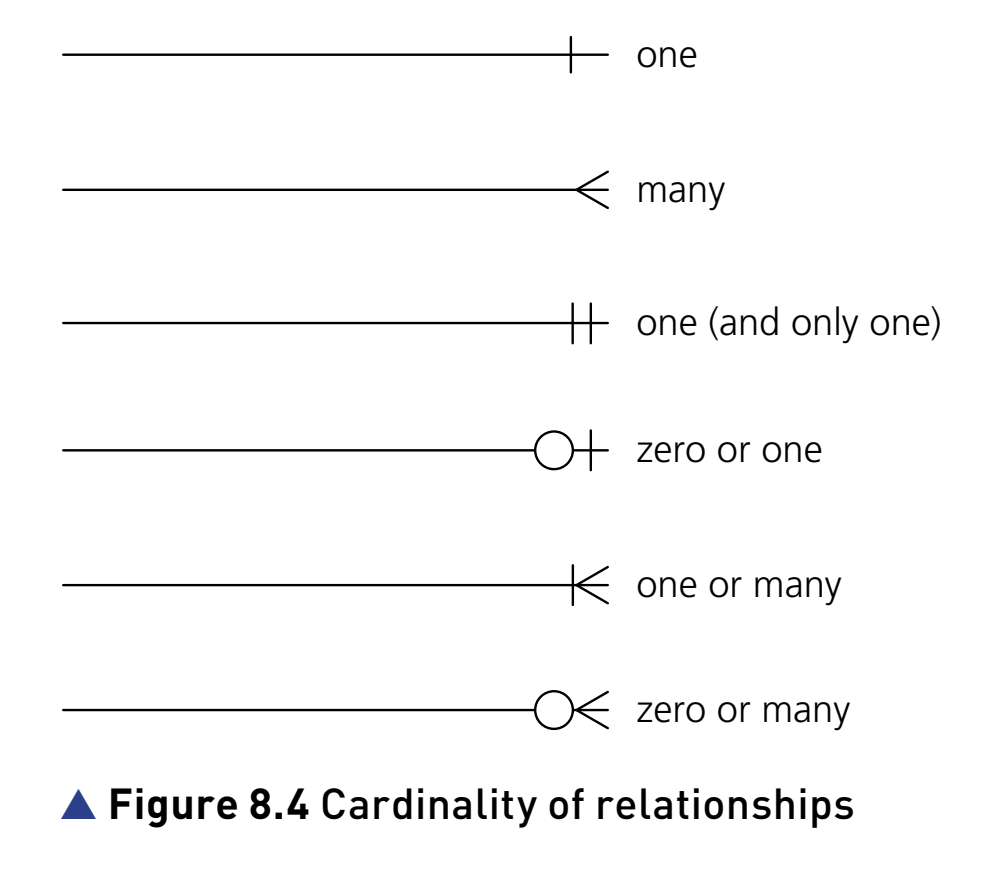
\includegraphics[width=200pt]{image.png}
    \end{center}
    

    \section{Normalisation}

    Ensures that database has integrity and that data redundancy is reduced. 

    \subsection{First Normalisation (1NF)}
    Entities don't have repeated groups/attributes.

    So you remove any repeated attributes from each table. Then you would create a separate table for these, and then link them with a foreign key. 

    \subsection{Second Normalisation (2NF)}
    Any non-key attributes depend only on the primary key, there're no partial dependencies.

    Partial dependencies happen when you're in a table and it has a composite primary key. But some of the attributes depend on only one specific part of the composite primary key, so for second normalisation you need to change this.

    We just make another table by breaking up the composite key, and storing one of the broken up keys and the matching datas into that new table. 

    \subsection{Third Normalisation (3NF)}
    All non-key values are independent. The table has no non-key dependencies.
    
    So here, if in a table there are attributes that depend on another key that's not the primary key, just make a separate table.

    \section{DBMS}

    Data modelling and data dictionary: data dictionary stores meta data about the database (table names, columns in each table, datatypes they contain). Data modelling shows the structure of data: eg E-R diagram, and logical schemas. Logical schemas shows the tables and attributes of a database.

    Use and and purpose of DBMS: 

    \begin{itemize}
        \item Developer Interface: allows users to write queries, and these queries are processed by $\textbf{query processer}$.
        \item Query Processor: DDL processor and DML compiler. 
    \end{itemize}


    \section{DDL and DML}
    Data Definition Language (DDL): Creates datastructures like tables and attributes.

    Data Manipulation Language (DML): Moves, modifies, deletes data in a database.

    \subsection{Data Definition Language}
    \begin{center}
        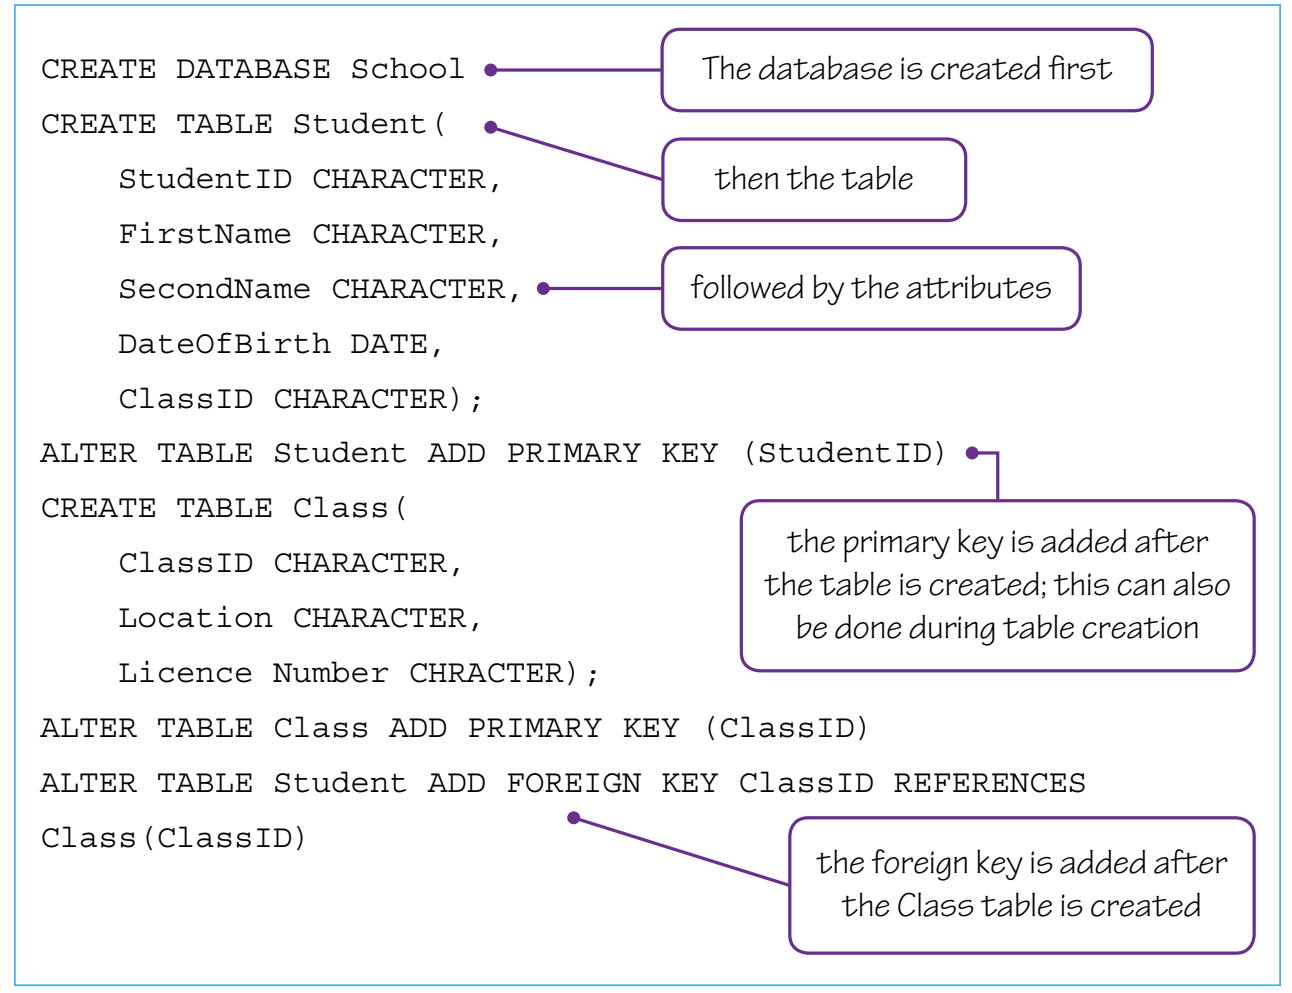
\includegraphics[width = 275pt]{Capture-2025-09-06-154943.png}
    \end{center}

    \subsection{Data Manipulation Language}
    \begin{center}
        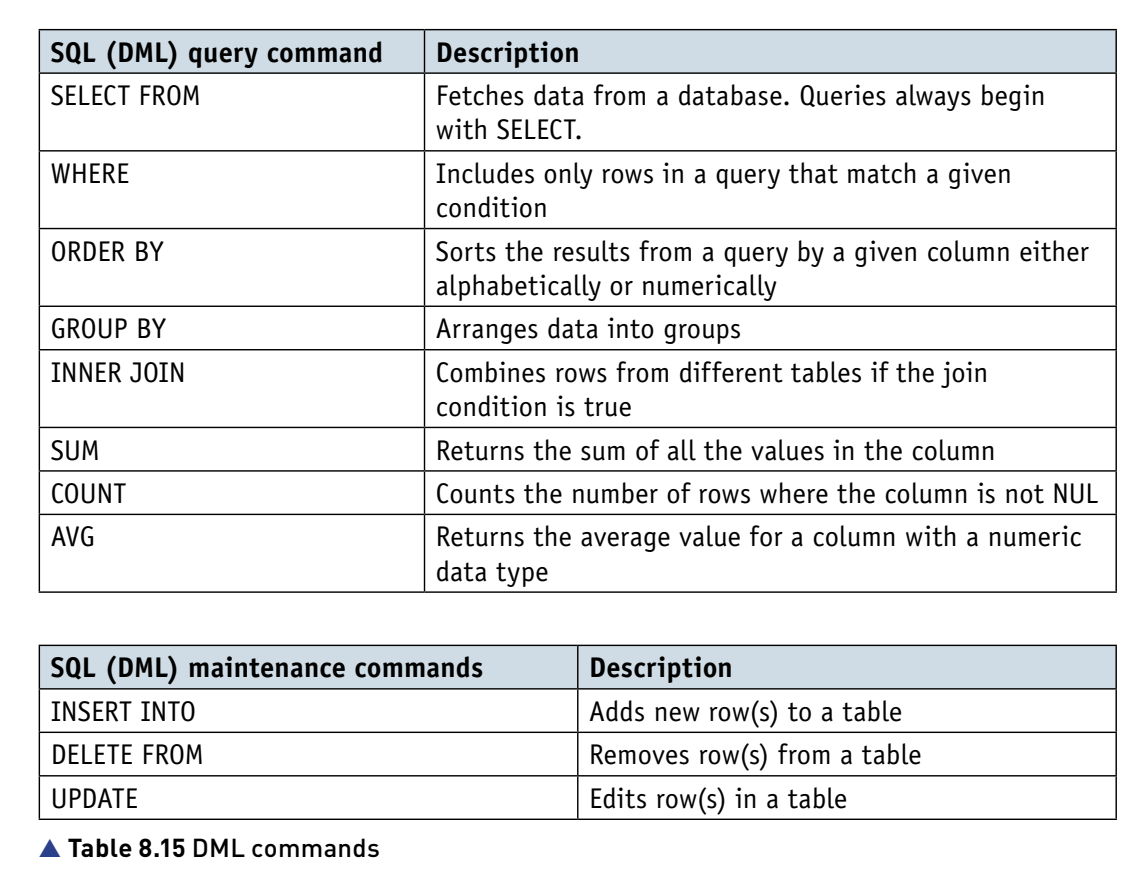
\includegraphics[width = 275pt]{Capture-2025-09-06-155844.png}
        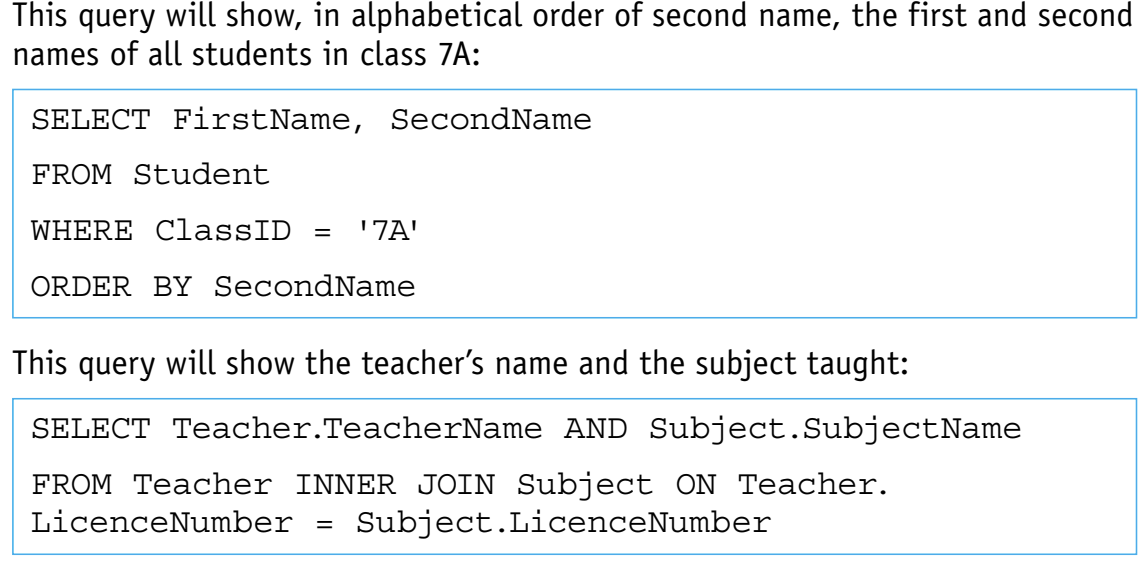
\includegraphics[width = 275pt]{image copy.png}
    \end{center}

    Note the INNER JOIN command in the examples: you're joining the columns from two distinct tables that have the same value. Syntax should be: 

    FROM Table1 INNER JOIN Table2 ON Table1.column1 = Table2.column2.

    Also, when using "INSERT INTO", the syntax is INSERT INTO table1 VALUES(value1, value2...)

    




    
\end{document}